% Options for packages loaded elsewhere
% Options for packages loaded elsewhere
\PassOptionsToPackage{unicode}{hyperref}
\PassOptionsToPackage{hyphens}{url}
%
\documentclass[
  ignorenonframetext,
  aspectratio=169,
  russian,
]{beamer}
\newif\ifbibliography
\usepackage{pgfpages}
\setbeamertemplate{caption}[numbered]
\setbeamertemplate{caption label separator}{: }
\setbeamercolor{caption name}{fg=normal text.fg}
\beamertemplatenavigationsymbolshorizontal
% remove section numbering
\setbeamertemplate{part page}{
  \centering
  \begin{beamercolorbox}[sep=16pt,center]{part title}
    \usebeamerfont{part title}\insertpart\par
  \end{beamercolorbox}
}
\setbeamertemplate{section page}{
  \centering
  \begin{beamercolorbox}[sep=12pt,center]{section title}
    \usebeamerfont{section title}\insertsection\par
  \end{beamercolorbox}
}
\setbeamertemplate{subsection page}{
  \centering
  \begin{beamercolorbox}[sep=8pt,center]{subsection title}
    \usebeamerfont{subsection title}\insertsubsection\par
  \end{beamercolorbox}
}
% Prevent slide breaks in the middle of a paragraph
\widowpenalties 1 10000
\raggedbottom
\AtBeginPart{
  \frame{\partpage}
}
\AtBeginSection{
  \ifbibliography
  \else
    \frame{\sectionpage}
  \fi
}
\AtBeginSubsection{
  \frame{\subsectionpage}
}
\usepackage{iftex}
\ifPDFTeX
  \usepackage[T1]{fontenc}
  \usepackage[utf8]{inputenc}
  \usepackage{textcomp} % provide euro and other symbols
\else % if luatex or xetex
  \usepackage{unicode-math} % this also loads fontspec
  \defaultfontfeatures{Scale=MatchLowercase}
  \defaultfontfeatures[\rmfamily]{Ligatures=TeX,Scale=1}
\fi
\usepackage{lmodern}

\ifPDFTeX\else
  % xetex/luatex font selection
\fi
% Use upquote if available, for straight quotes in verbatim environments
\IfFileExists{upquote.sty}{\usepackage{upquote}}{}
\IfFileExists{microtype.sty}{% use microtype if available
  \usepackage[]{microtype}
  \UseMicrotypeSet[protrusion]{basicmath} % disable protrusion for tt fonts
}{}


\usepackage{longtable,booktabs,array}
\newcounter{none} % for unnumbered tables
\usepackage{calc} % for calculating minipage widths
\usepackage{caption}
% Make caption package work with longtable
\makeatletter
\def\fnum@table{\tablename~\thetable}
\makeatother
\usepackage{graphicx}
\makeatletter
\newsavebox\pandoc@box
\newcommand*\pandocbounded[1]{% scales image to fit in text height/width
  \sbox\pandoc@box{#1}%
  \Gscale@div\@tempa{\textheight}{\dimexpr\ht\pandoc@box+\dp\pandoc@box\relax}%
  \Gscale@div\@tempb{\linewidth}{\wd\pandoc@box}%
  \ifdim\@tempb\p@<\@tempa\p@\let\@tempa\@tempb\fi% select the smaller of both
  \ifdim\@tempa\p@<\p@\scalebox{\@tempa}{\usebox\pandoc@box}%
  \else\usebox{\pandoc@box}%
  \fi%
}
% Set default figure placement to htbp
\def\fps@figure{htbp}
\makeatother



\ifLuaTeX
\usepackage[bidi=basic,shorthands=off,provide=*]{babel}
\else
\usepackage[bidi=default,shorthands=off,provide=*]{babel}
\fi
\ifLuaTeX
  \usepackage{selnolig} % disable illegal ligatures
\fi


\setlength{\emergencystretch}{3em} % prevent overfull lines

\providecommand{\tightlist}{%
  \setlength{\itemsep}{0pt}\setlength{\parskip}{0pt}}



 

\usepackage[]{csquotes}

\IfFileExists{plex-otf.sty}{
  %% Full TeXlive
  % \usepackage[%
  %   % math,
  %   RM={Scale=0.94},SS={Scale=0.94},SScon={Scale=0.94},TT={Scale=MatchLowercase,FakeStretch=0.9},DefaultFeatures={Ligatures=Common}
  % ]{plex-otf}
}{
  %% TinyTeX
  \usepackage{libertine}
}

%%% Load theme
% https://deic.uab.cat/~iblanes/beamer_gallery/
\IfFileExists{beamerthemegotham.sty}{
  %% Full TeXlive
  \usetheme{gotham}
  \gothamset{
    numbering=totalpagenumber,
    parttocframe default=off,
    sectiontocframe default=off,
    subsectiontocframe default=off,
  }
}{
  %% TinyTeX
  \usetheme{Madrid}
}
\makeatletter
\@ifpackageloaded{caption}{}{\usepackage{caption}}
\AtBeginDocument{%
\ifdefined\contentsname
  \renewcommand*\contentsname{Содержание}
\else
  \newcommand\contentsname{Содержание}
\fi
\ifdefined\listfigurename
  \renewcommand*\listfigurename{Список иллюстраций}
\else
  \newcommand\listfigurename{Список иллюстраций}
\fi
\ifdefined\listtablename
  \renewcommand*\listtablename{Список таблиц}
\else
  \newcommand\listtablename{Список таблиц}
\fi
\ifdefined\figurename
  \renewcommand*\figurename{Рисунок}
\else
  \newcommand\figurename{Рисунок}
\fi
\ifdefined\tablename
  \renewcommand*\tablename{Таблица}
\else
  \newcommand\tablename{Таблица}
\fi
}
\@ifpackageloaded{float}{}{\usepackage{float}}
\floatstyle{ruled}
\@ifundefined{c@chapter}{\newfloat{codelisting}{h}{lop}}{\newfloat{codelisting}{h}{lop}[chapter]}
\floatname{codelisting}{Список}
\newcommand*\listoflistings{\listof{codelisting}{Листинги}}
\makeatother
\makeatletter
\makeatother
\makeatletter
\@ifpackageloaded{caption}{}{\usepackage{caption}}
\@ifpackageloaded{subcaption}{}{\usepackage{subcaption}}
\makeatother

\usepackage{bookmark}
\IfFileExists{xurl.sty}{\usepackage{xurl}}{} % add URL line breaks if available
\urlstyle{same}
% fallback for those not using the hyperref driver hyperxmp:
\makeatletter
\@ifundefined{xmpquote}{\newcommand{\xmpquote}[1]{#1}}{}
\makeatother
\hypersetup{
  pdftitle={Лабораторная работа №2},
  pdfauthor={Кудякова София Андреевна},
  pdflang={ru},
  hidelinks,
  pdfcreator={LaTeX via pandoc}}


\title{\texorpdfstring{Лабораторная работа №2}{Лабораторная работа №2}}
\subtitle{\texorpdfstring{Имитационное
моделирование}{Имитационное моделирование}}
\author{Кудякова София Андреевна}
\date{2026-08-26}

\begin{document}
\frame{\titlepage}

\renewcommand*\contentsname{Содержание}
\begin{frame}[allowframebreaks]
  \frametitle{Содержание}
  \setcounter{tocdepth}{1}
  \tableofcontents
\end{frame}
\setcounter{tocdepth}{1}
\tableofcontents
}

\section{Вводная
часть}\label{ux432ux432ux43eux434ux43dux430ux44f-ux447ux430ux441ux442ux44c}

\begin{frame}{Цель и задачи}
\protect\phantomsection\label{ux446ux435ux43bux44c-ux438-ux437ux430ux434ux430ux447ux438}
\textbf{Цель:} познакомиться с моделями SIR и Лотки--Вольтерры,
реализовать их средствами Julia, выполнить моделирование и исследовать
влияние параметров.

\textbf{Задачи:}

\begin{itemize}[<+->]
\tightlist
\item
  реализовать модели SIR и Лотки--Вольтерры;
\item
  преобразовать код в литературный стиль;
\item
  сгенерировать Julia-скрипт, Jupyter Notebook и Quarto-документ;
\item
  выполнить параметрическое исследование моделей;
\item
  проанализировать полученные результаты.
\end{itemize}
\end{frame}

\begin{frame}{Модель SIR}
\protect\phantomsection\label{ux43cux43eux434ux435ux43bux44c-sir}
Группы населения: \textbf{S} --- восприимчивые, \textbf{I} ---
инфицированные, \textbf{R} --- выздоровевшие.

\[
\frac{dS}{dt} = -\beta c \frac{SI}{N}, \quad
\frac{dI}{dt} = \beta c \frac{SI}{N} - \gamma I, \quad
\frac{dR}{dt} = \gamma I
\]

Базовое репродуктивное число:

\[
R_0 = \frac{\beta c}{\gamma}
\]
\end{frame}

\begin{frame}{Модель Лотки--Вольтерры}
\protect\phantomsection\label{ux43cux43eux434ux435ux43bux44c-ux43bux43eux442ux43aux438ux432ux43eux43bux44cux442ux435ux440ux440ux44b}
\(x\) --- численность жертв, \(y\) --- численность хищников.

\[
\frac{dx}{dt} = \alpha x - \beta xy, \qquad
\frac{dy}{dt} = \delta xy - \gamma y
\]

Модель описывает циклическое изменение численности двух
взаимодействующих популяций.
\end{frame}

\section{Подготовка
проекта}\label{ux43fux43eux434ux433ux43eux442ux43eux432ux43aux430-ux43fux440ux43eux435ux43aux442ux430}

\begin{frame}{Структура проекта}
\protect\phantomsection\label{ux441ux442ux440ux443ux43aux442ux443ux440ux430-ux43fux440ux43eux435ux43aux442ux430}
Организация Julia-проекта с отдельными каталогами для кода, notebooks,
документов Quarto и графиков.

\begin{figure}

\centering{


\includegraphics[width=0.7\linewidth,height=\textheight,keepaspectratio]{image/1.png}

}

\caption{\label{fig-001}Структура рабочего проекта}

\end{figure}%
\end{frame}

\begin{frame}{Проверка окружения}
\protect\phantomsection\label{ux43fux440ux43eux432ux435ux440ux43aux430-ux43eux43aux440ux443ux436ux435ux43dux438ux44f}
Установлены необходимые пакеты Julia, выполнена проверка рабочего
окружения.

\begin{figure}

\centering{


\includegraphics[width=0.7\linewidth,height=\textheight,keepaspectratio]{image/2.png}

}

\caption{\label{fig-002}Проверка рабочего окружения}

\end{figure}%
\end{frame}

\section{Модель SIR}\label{ux43cux43eux434ux435ux43bux44c-sir-1}

\begin{frame}{Базовая реализация}
\protect\phantomsection\label{ux431ux430ux437ux43eux432ux430ux44f-ux440ux435ux430ux43bux438ux437ux430ux446ux438ux44f}
Параметры модели:

\[
\beta = 0.05,\quad c = 10.0,\quad \gamma = 0.25
\]

Начальные условия:

\[
S_0 = 990,\quad I_0 = 10,\quad R_0 = 0
\]

Базовое репродуктивное число: \(R_0 = 2\).

\begin{figure}

\centering{


\includegraphics[width=0.7\linewidth,height=\textheight,keepaspectratio]{image/3.png}

}

\caption{\label{fig-003}Результат выполнения модели SIR}

\end{figure}%
\end{frame}

\begin{frame}{Результаты базового эксперимента}
\protect\phantomsection\label{ux440ux435ux437ux443ux43bux44cux442ux430ux442ux44b-ux431ux430ux437ux43eux432ux43eux433ux43e-ux44dux43aux441ux43fux435ux440ux438ux43cux435ux43dux442ux430}
\begin{itemize}[<+->]
\tightlist
\item
  Максимальное число инфицированных: \(I_{\max} = 154.8\)
\item
  Пик эпидемии: \(t_{\text{peak}} \approx 19.1\) дня
\item
  Итоговое число выздоровевших: \(R(\infty) = 775.7\)
\end{itemize}
\end{frame}

\begin{frame}{Графики модели SIR}
\protect\phantomsection\label{ux433ux440ux430ux444ux438ux43aux438-ux43cux43eux434ux435ux43bux438-sir}
\begin{figure}

\centering{


\includegraphics[width=0.7\linewidth,height=\textheight,keepaspectratio]{image/4.png}

}

\caption{\label{fig-004}Динамика восприимчивых, инфицированных и
выздоровевших}

\end{figure}%

\begin{figure}

\centering{


\includegraphics[width=0.7\linewidth,height=\textheight,keepaspectratio]{image/7.png}

}

\caption{\label{fig-007}Фазовый портрет модели SIR}

\end{figure}%
\end{frame}

\begin{frame}{Параметрическое исследование SIR}
\protect\phantomsection\label{ux43fux430ux440ux430ux43cux435ux442ux440ux438ux447ux435ux441ux43aux43eux435-ux438ux441ux441ux43bux435ux434ux43eux432ux430ux43dux438ux435-sir}
Рассмотрены значения:

\[
\beta \in \{0.03,\;0.05,\;0.07\}
\]

{\def\LTcaptype{none} % do not increment counter
\begin{longtable}[]{@{}llll@{}}
\toprule\noalign{}
\(\beta\) & \(I_{\max}\) & \(t_{\text{peak}}\) & \(R_{\text{final}}\) \\
\midrule\noalign{}
\endhead
0.03 & 22.7 & 36.5 & 187.8 \\
0.05 & 154.8 & 19.1 & 775.7 \\
0.07 & 276.5 & 11.0 & 923.1 \\
\bottomrule\noalign{}
\end{longtable}
}
\end{frame}

\begin{frame}{Результат параметрического исследования}
\protect\phantomsection\label{ux440ux435ux437ux443ux43bux44cux442ux430ux442-ux43fux430ux440ux430ux43cux435ux442ux440ux438ux447ux435ux441ux43aux43eux433ux43e-ux438ux441ux441ux43bux435ux434ux43eux432ux430ux43dux438ux44f}
Увеличение \(\beta\) ускоряет распространение инфекции и увеличивает
масштаб эпидемии.

\begin{figure}

\centering{


\includegraphics[width=0.7\linewidth,height=\textheight,keepaspectratio]{image/9.png}

}

\caption{\label{fig-009}Параметрическое исследование модели SIR}

\end{figure}%
\end{frame}

\begin{frame}{Производные файлы модели SIR}
\protect\phantomsection\label{ux43fux440ux43eux438ux437ux432ux43eux434ux43dux44bux435-ux444ux430ux439ux43bux44b-ux43cux43eux434ux435ux43bux438-sir}
Из литературного кода сгенерированы:

\begin{itemize}[<+->]
\tightlist
\item
  Julia-скрипт;
\item
  Jupyter Notebook;
\item
  документ Quarto.
\end{itemize}

\begin{figure}

\centering{


\includegraphics[width=0.7\linewidth,height=\textheight,keepaspectratio]{image/10.png}

}

\caption{\label{fig-010}Генерация производных файлов модели SIR}

\end{figure}%
\end{frame}

\section{Модель
Лотки--Вольтерры}\label{ux43cux43eux434ux435ux43bux44c-ux43bux43eux442ux43aux438ux432ux43eux43bux44cux442ux435ux440ux440ux44b-1}

\begin{frame}{Базовая реализация}
\protect\phantomsection\label{ux431ux430ux437ux43eux432ux430ux44f-ux440ux435ux430ux43bux438ux437ux430ux446ux438ux44f-1}
Параметры модели:

\[
\alpha = 0.1,\quad \beta = 0.02,\quad \delta = 0.01,\quad \gamma = 0.3
\]

Начальные условия: \(x_0 = 40\), \(y_0 = 9\).

Стационарная точка: \(x^* = 30\), \(y^* = 5\).

\begin{figure}

\centering{


\includegraphics[width=0.7\linewidth,height=\textheight,keepaspectratio]{image/11.png}

}

\caption{\label{fig-011}Результат выполнения модели Лотки--Вольтерры}

\end{figure}%
\end{frame}

\begin{frame}{Графики модели Лотки--Вольтерры}
\protect\phantomsection\label{ux433ux440ux430ux444ux438ux43aux438-ux43cux43eux434ux435ux43bux438-ux43bux43eux442ux43aux438ux432ux43eux43bux44cux442ux435ux440ux440ux44b}
\begin{figure}

\centering{


\includegraphics[width=0.7\linewidth,height=\textheight,keepaspectratio]{image/12.png}

}

\caption{\label{fig-012}Динамика численности жертв и хищников}

\end{figure}%

\begin{figure}

\centering{


\includegraphics[width=0.7\linewidth,height=\textheight,keepaspectratio]{image/13.png}

}

\caption{\label{fig-013}Фазовый портрет модели Лотки--Вольтерры}

\end{figure}%
\end{frame}

\begin{frame}{Параметрическое исследование Лотки--Вольтерры}
\protect\phantomsection\label{ux43fux430ux440ux430ux43cux435ux442ux440ux438ux447ux435ux441ux43aux43eux435-ux438ux441ux441ux43bux435ux434ux43eux432ux430ux43dux438ux435-ux43bux43eux442ux43aux438ux432ux43eux43bux44cux442ux435ux440ux440ux44b}
Рассмотрены значения:

\[
\alpha \in \{0.05,\;0.1,\;0.2\}
\]

Изменение \(\alpha\) влияет на скорость роста популяции жертв и, как
следствие, на динамику хищников.

\begin{figure}

\centering{


\includegraphics[width=0.7\linewidth,height=\textheight,keepaspectratio]{image/17.png}

}

\caption{\label{fig-017}Результаты параметрического исследования модели
Лотки--Вольтерры}

\end{figure}%
\end{frame}

\begin{frame}{Производные файлы модели Лотки--Вольтерры}
\protect\phantomsection\label{ux43fux440ux43eux438ux437ux432ux43eux434ux43dux44bux435-ux444ux430ux439ux43bux44b-ux43cux43eux434ux435ux43bux438-ux43bux43eux442ux43aux438ux432ux43eux43bux44cux442ux435ux440ux440ux44b}
Из литературного кода сгенерированы Julia-скрипт, Jupyter Notebook и
документ Quarto.

\begin{figure}

\centering{


\includegraphics[width=0.7\linewidth,height=\textheight,keepaspectratio]{image/18.png}

}

\caption{\label{fig-018}Генерация производных файлов модели
Лотки--Вольтерры}

\end{figure}%
\end{frame}

\section{Jupyter Notebook}\label{jupyter-notebook}

\begin{frame}{Выполнение Notebook}
\protect\phantomsection\label{ux432ux44bux43fux43eux43bux43dux435ux43dux438ux435-notebook}
Результат выполнения Jupyter Notebook для обеих моделей:

\begin{figure}

\centering{

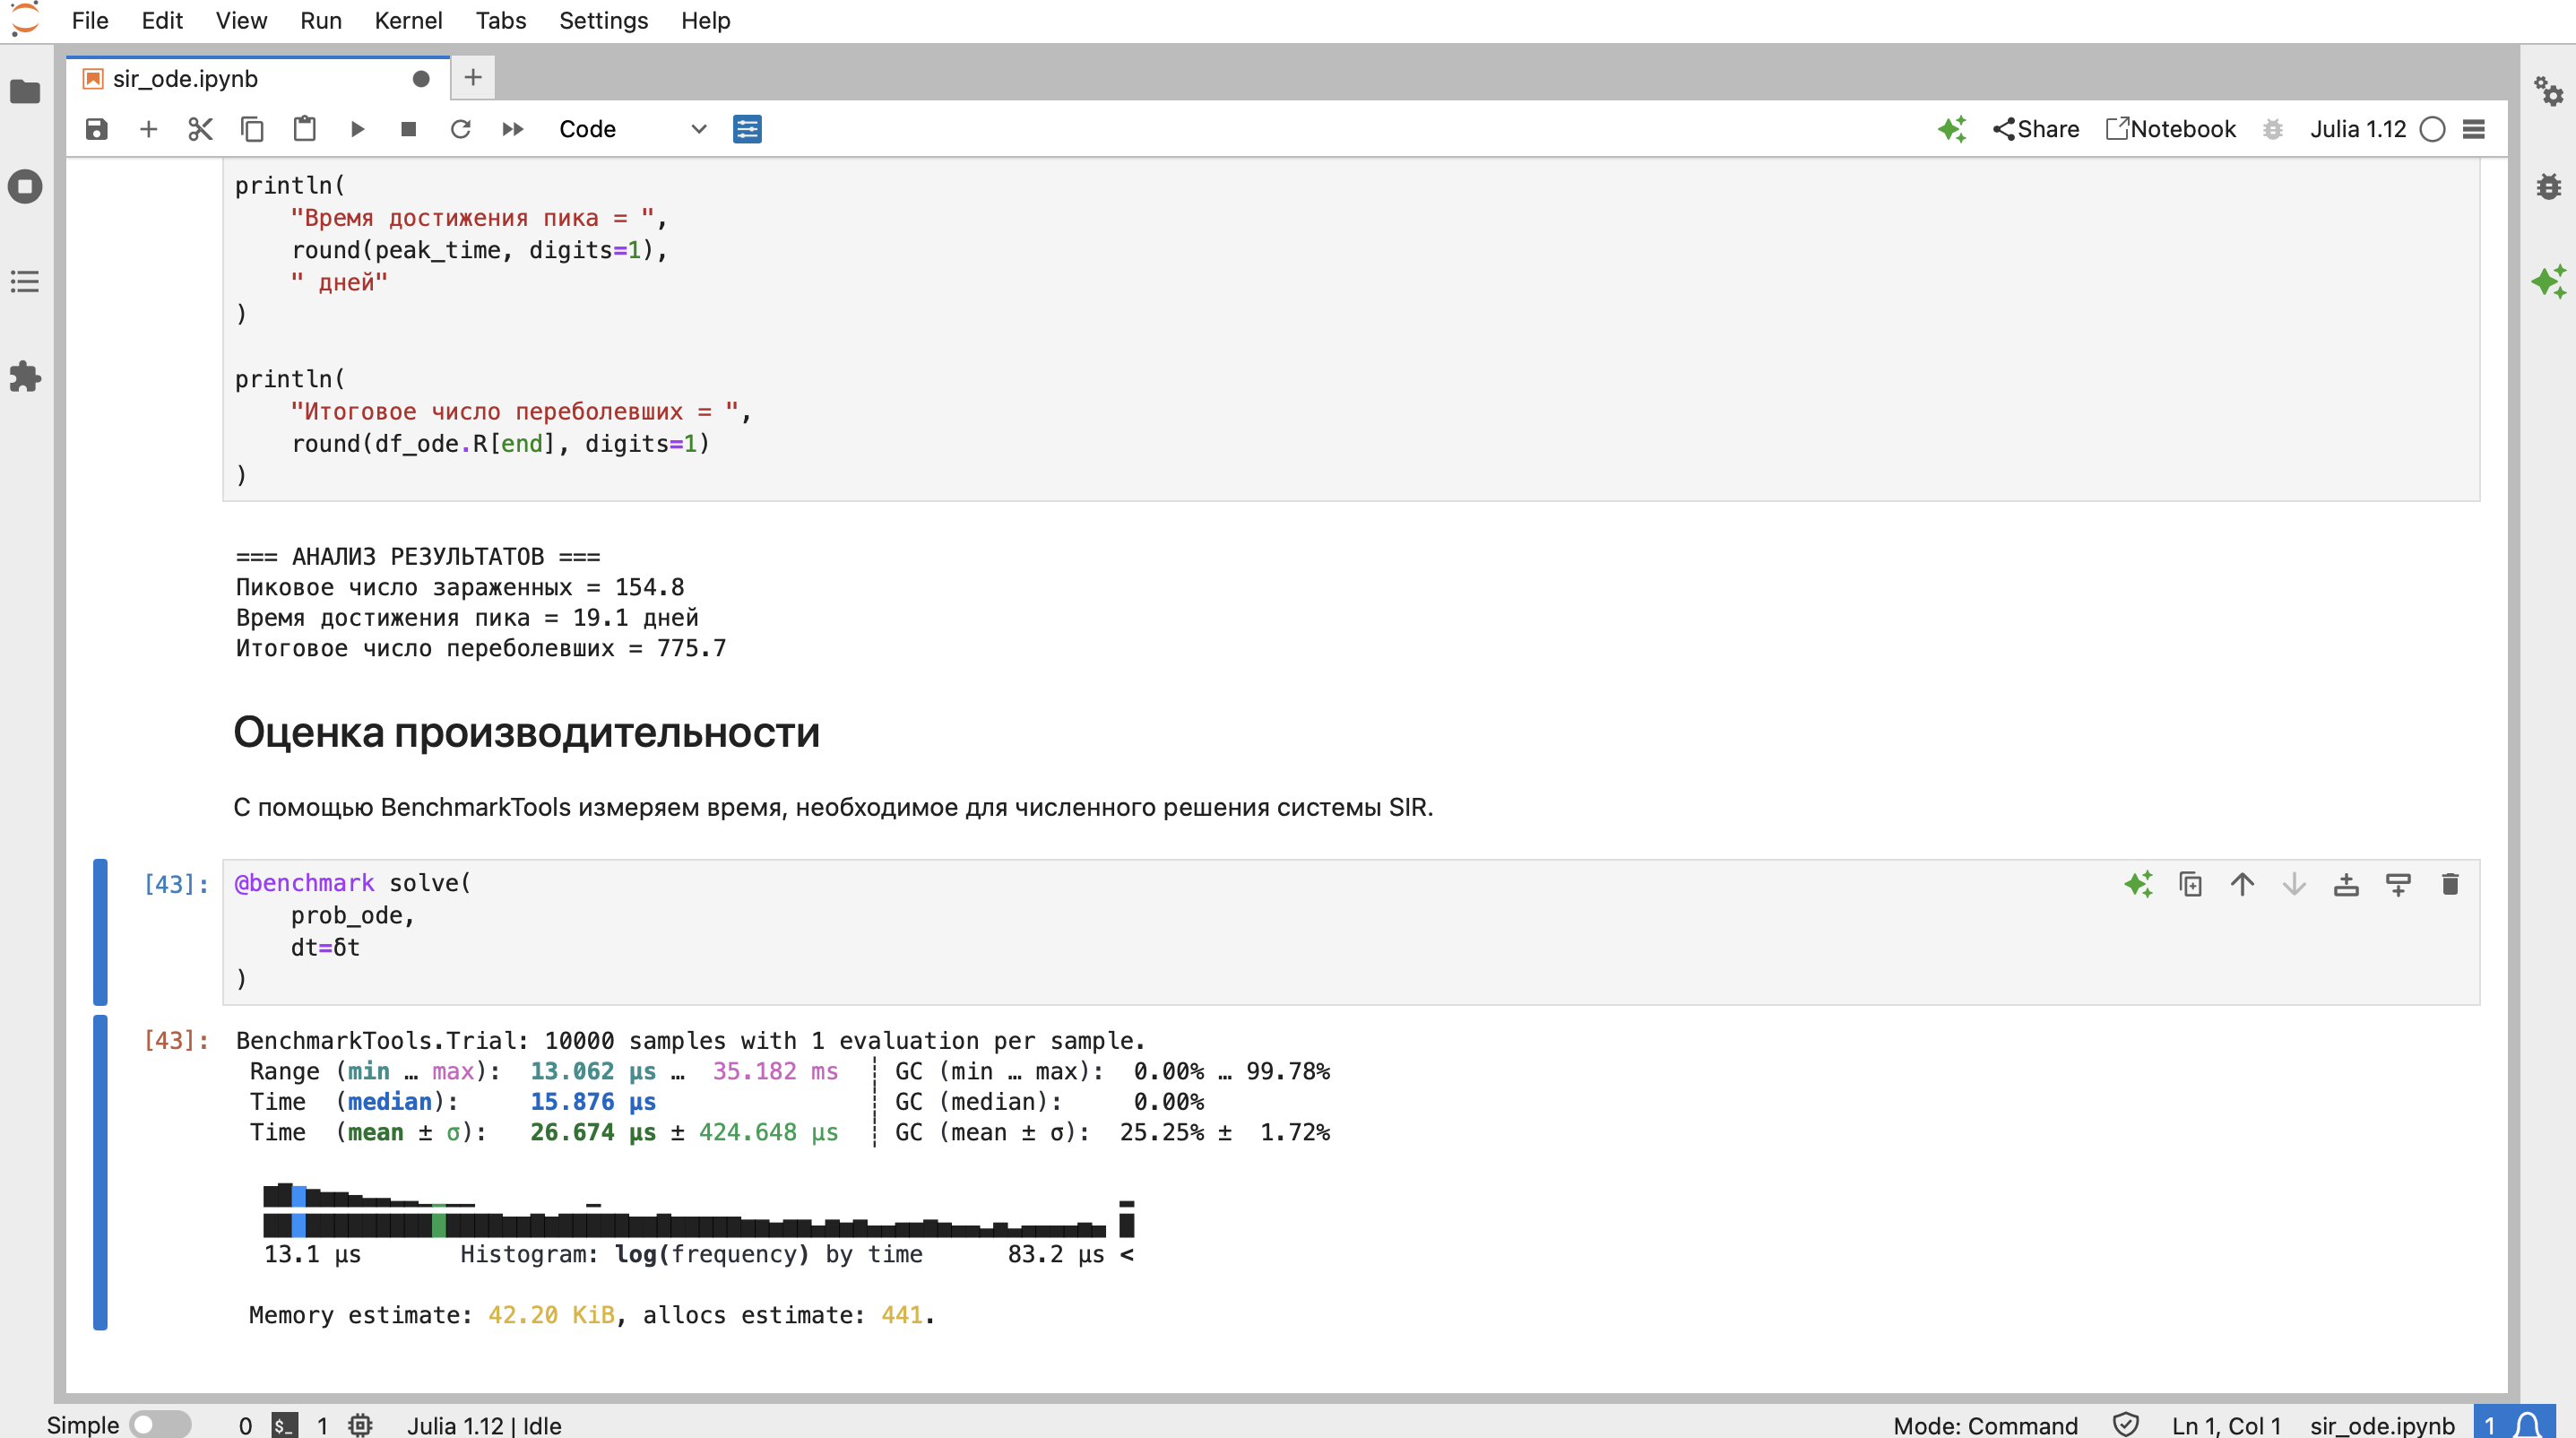
\includegraphics[width=0.7\linewidth,height=\textheight,keepaspectratio]{image/19.png}

}

\caption{\label{fig-019}Результат выполнения Jupyter Notebook модели
SIR}

\end{figure}%

\begin{figure}

\centering{

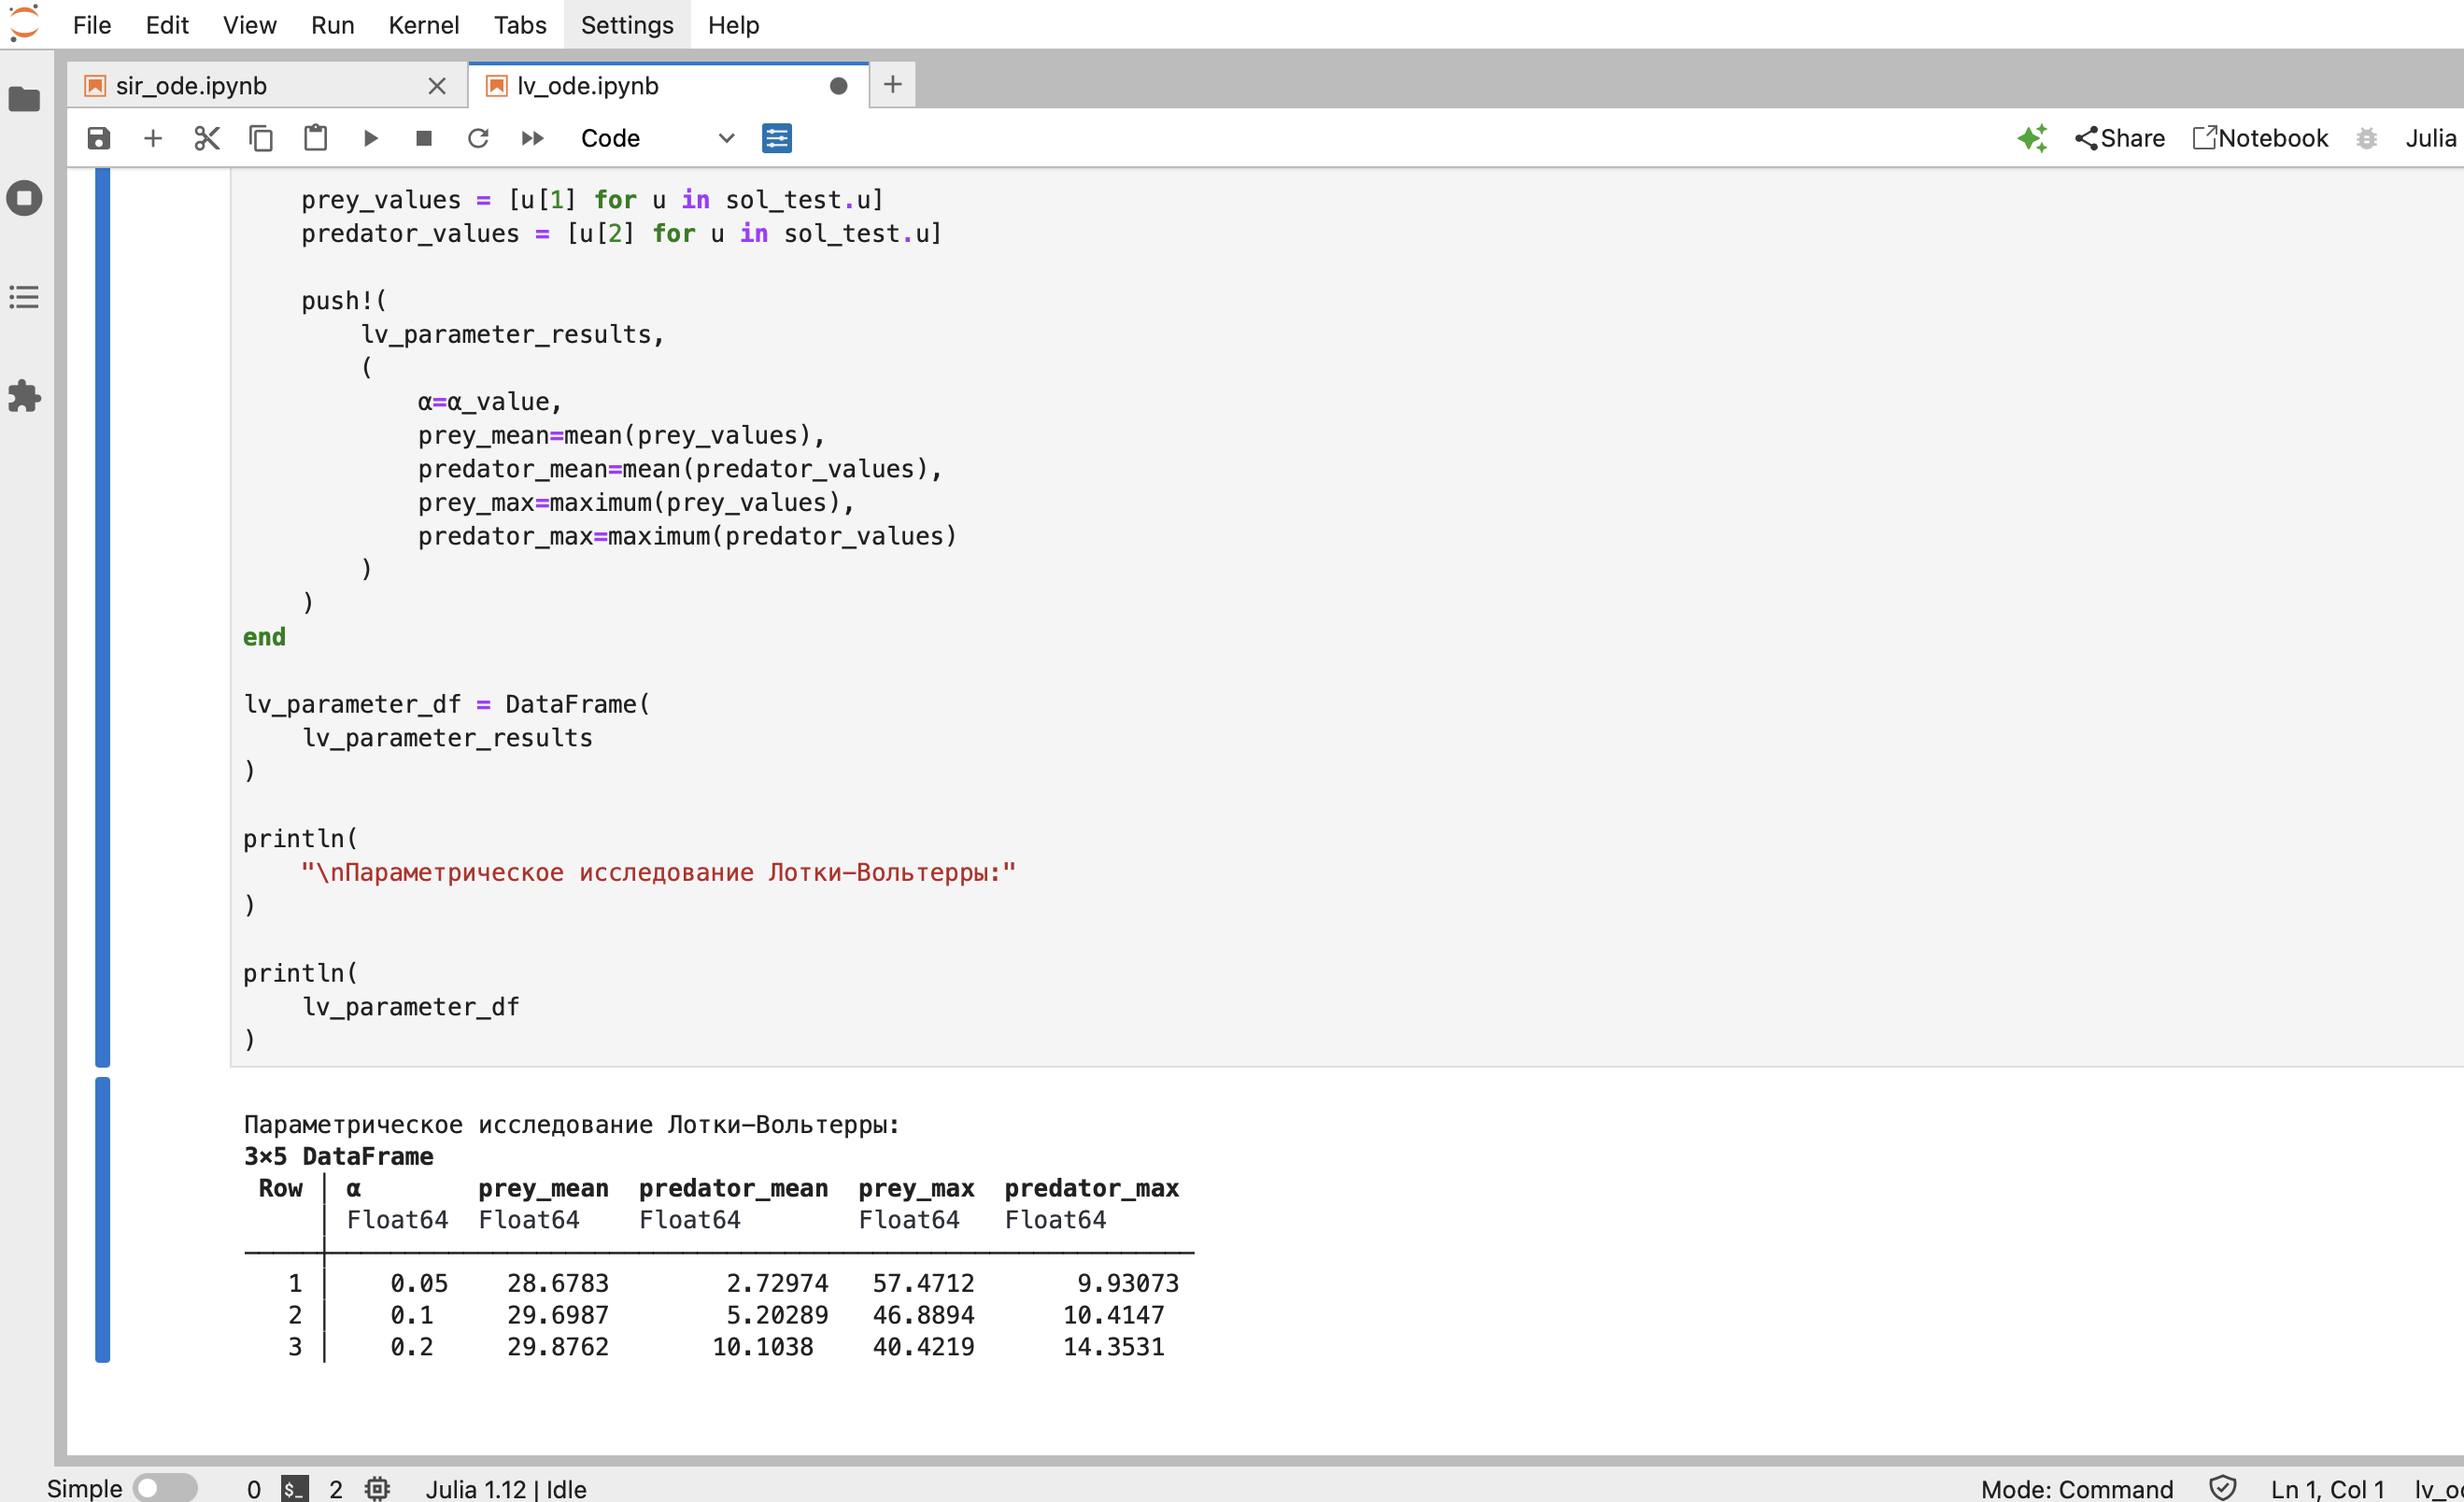
\includegraphics[width=0.7\linewidth,height=\textheight,keepaspectratio]{image/20.png}

}

\caption{\label{fig-020}Результат выполнения Jupyter Notebook модели
Лотки--Вольтерры}

\end{figure}%
\end{frame}

\section{Результаты}\label{ux440ux435ux437ux443ux43bux44cux442ux430ux442ux44b}

\begin{frame}{Анализ модели SIR}
\protect\phantomsection\label{ux430ux43dux430ux43bux438ux437-ux43cux43eux434ux435ux43bux438-sir}
\begin{itemize}[<+->]
\tightlist
\item
  \(R_0 = 2\) при базовых параметрах
\item
  Пик инфицированных \(\approx 154.8\) человек на 19.1-й день
\item
  Увеличение \(\beta\) ускоряет и усиливает эпидемию
\end{itemize}
\end{frame}

\begin{frame}{Анализ модели Лотки--Вольтерры}
\protect\phantomsection\label{ux430ux43dux430ux43bux438ux437-ux43cux43eux434ux435ux43bux438-ux43bux43eux442ux43aux438ux432ux43eux43bux44cux442ux435ux440ux440ux44b}
\begin{itemize}[<+->]
\tightlist
\item
  Стационарная точка \((x^*, y^*) = (30, 5)\)
\item
  Циклические изменения численности жертв и хищников
\item
  Изменение \(\alpha\) влияет на скорость роста жертв и динамику
  хищников
\end{itemize}
\end{frame}

\begin{frame}{Выводы}
\protect\phantomsection\label{ux432ux44bux432ux43eux434ux44b}
\begin{itemize}[<+->]
\tightlist
\item
  Реализованы модели SIR и Лотки--Вольтерры на Julia
\item
  Проведено параметрическое исследование обеих моделей
\item
  Освоены литературное программирование, генерация Jupyter Notebook и
  Quarto-документов
\item
  Получены количественные зависимости влияния параметров на динамику
  моделей
\end{itemize}
\end{frame}




\end{document}
